\documentclass[12pt]{report}
\usepackage[utf8]{inputenc}
\usepackage{graphicx}
\usepackage{float}
\usepackage{hyperref}
\usepackage[left=2cm,right=2cm,top=2cm,bottom=2cm]{geometry}
\usepackage{listings}

\begin{document}
\begin{titlepage}

\newcommand{\HRule}{\rule{\linewidth}{0.5mm}} % Defines a new command for the horizontal lines, change thickness here

\center 
\HRule \\[0.4cm]
{ \huge \bfseries User Guide: \\Representation and relative positioning from visual information}\\[0.4cm]
\HRule \\[1.5cm]

\begin{minipage}{0.4\textwidth}
	\begin{flushleft} \large
		\emph{Submitted by:}\\
		\textsc{Asma BRAZI}
	\end{flushleft}
\end{minipage}
~
\begin{minipage}{0.4\textwidth}
	\begin{flushright} \large
		\emph{Supervised by:} \\
		\textsc{Cédric HERPSON}\\
	\end{flushright}
\end{minipage}\\[4cm]


{\large Laboratory of Computer Sciences, Paris 6 \\ Sorbonne University - Faculty of Sciences and Engineering}\\[3cm] 
{\large June - July 2019 }\\[3cm] 

\includegraphics[width=0.6\textwidth]{logo.png}\\[1cm] 
\vfill % Fill the rest of the page with whitespace

\end{titlepage}
\tableofcontents
\chapter{Introduction}
\paragraph{}
This document represents a guide for users. It is necessary to be consulted to ensure a proper configuration of the environment. It is designed to:
\begin{itemize}
    \item Enumerate the different hardware and software prerequisites.
    \item Provide a step-by-step instructions to establish the environment configuration.
    \item Present a brief scenario of how the application runs.
\end{itemize}
\chapter{Getting started}
\paragraph{}
We present in this section the necessary equipment for the use of our application. Also, we specify the essential programs to install.
\section{Hardware prerequisites}
\paragraph{}
The global system can be seen as two independent physical subsystems in interaction. The first one is composed of a computer, and the second one is what we call the autonomous robot. and whose list of components is showed in the figure below.
\begin{figure}[H]
	\begin{center}
		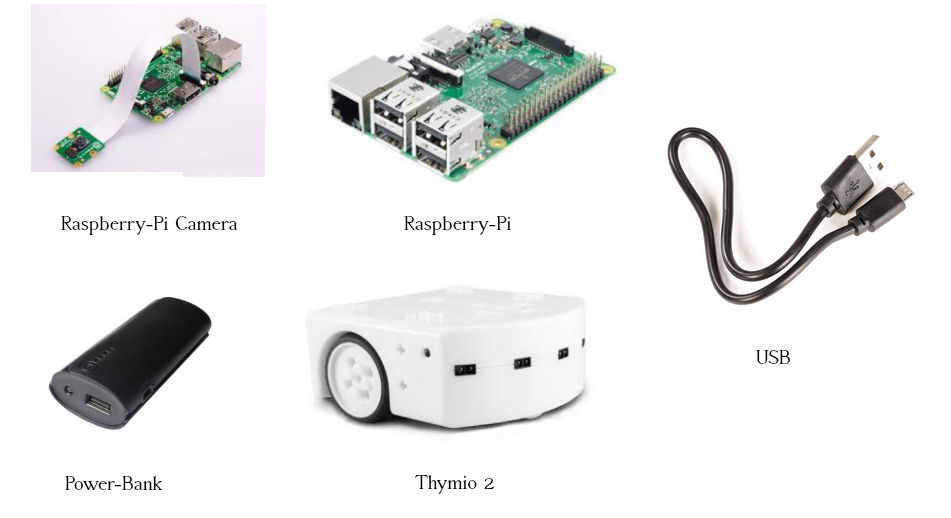
\includegraphics[scale=0.6]{comp.png}
		\caption{The components of the autonomous robot}
	\end{center}
\end{figure}
\paragraph{}
The computer and the autonomous robot are exchanging via Wi-Fi. Nevertheless, the autonomous robot's components are connecting with cables. 
So, to connect the autonomous robot's components, we insert the Raspberry-Pi Camera's cable by into the Raspberry-Pi, so as that the cable is placed between Ethernet and HDMI ports, see Fig 2.2. 

\begin{figure}[H]
	\begin{center}
		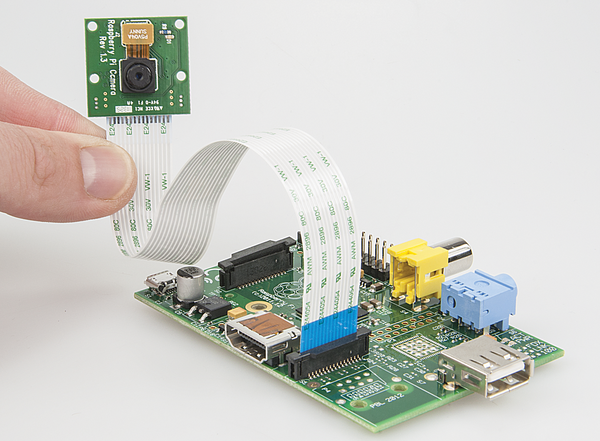
\includegraphics[scale=0.8]{campirasp.png}
		\caption{The connection of the Raspberry-Pi camera }
	\end{center}
\end{figure}
\paragraph{}
Then we connect the Thymio to the Raspberry-Pi with a cable. Finally, in order to power the Raspberry-Pi, we use the power-bank which is connected to it with USB. see Fig 2.3.
\begin{figure}[H]
	\begin{center}
		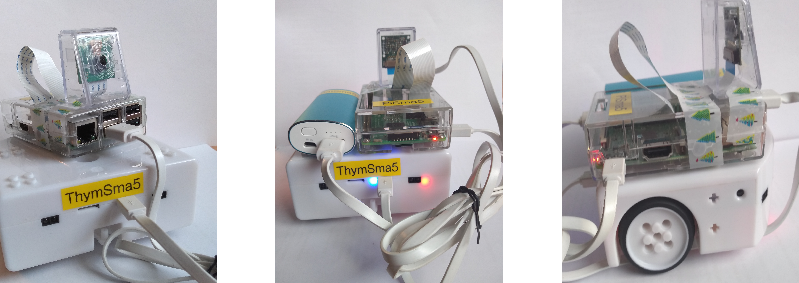
\includegraphics[scale=0.8]{robot_comp.png}
		\caption{The connected autonomous robot's components}
	\end{center}
\end{figure}
\section{OS/Software prerequisites}
\paragraph{}
We need several programs for both subsystems to be able to launch the application. The programs that we have to install on the computer are:
\begin{itemize}
	\item Java 8.
	\item Java IDE.
	\item JMonkey Engine.
\end{itemize}
\paragraph{}
Then those to install on the Raspberry-Pi are:
\begin{itemize}
	\item Python 3 and Pip 3.
    \item OpenCV.
    \item Asebamedulla.
\end{itemize}
Then, those to install on the computer are:

\paragraph{}
We begin with the set of programs to install on the computer. 
\subsection{Java 8}
\paragraph{}
Java can be installed with the following commands:

\begin{itemize}
	\item Go to the website \url{https://www.java.com/fr/download/linux_manual.jsp}
	\item Download the version corresponding to your OS (64x or 32x)
	\item The complete instructions to install it are available on the same web page.They are available by clicking on the button \emph{instructions} beside your the file to download.
	\item Go to the website \url{https://www.oracle.com/technetwork/java/javase/downloads/index.html}
	\item Download the latest version of JDK available.
	\item The installation instructions can been consulted on the same web page.
\end{itemize}


\subsection{Java IDE}
\paragraph{}
There are many Java IDE that may be used (IntelliJ IDEA, Eclipse, Netbeans, etc). In our project scope, we use Eclipse 2019-03. The following steps indicate how to install this IDE: 

\begin{itemize}
	\item Go to the website \url{https://www.eclipse.org/downloads/}
	\item Download the version of Eclipse IDE corresponding to your OS (64x or 32x)
	\item Extract the downloaded archive, open the extracted directory and launch \emph{eclipse-inst}
	\item Now, click on \emph{Eclipse IDE for Java Developers} 
	\item The followed instructions ask for the installation folder and the environment configuration (Eclipse's theme, etc), an installation by default can be done too.
\end{itemize}

\subsection{JMonkey Engine}
\paragraph{}
JMonkey Engine can be installed with the following commands:

\begin{itemize}
	\item Go to the website \url{https://github.com/jMonkeyEngine/sdk/releases}
	\item Download the latest stable version corresponding to your OS (64x or 32x).
	\item Open a terminal and execute the command \emph{sudo ./jmonkeyplatform-linux-*}
	\item The followed instructions ask for the installation folder and the environment configuration (Eclipse's theme, etc), an installation by default can be done too.
\end{itemize}


\subsection{Python 3}
\paragraph{}
Python can be installed with the following commands:

\begin{itemize}
	\item \emph{sudo apt-get update}
	\item \emph{sudo apt-get install python3.6}
\end{itemize}
The following command is used to verify if Python has been correctly installed: \emph{python3 - -version}

\subsection{Pip 3}
\paragraph{}
Pip can be installed with the following commands:
\begin{itemize}
	\item \emph{sudo apt-get update}
	\item \emph{sudo apt install python3-pip}
\end{itemize}
The following command is used to verify if Pip has been correctly installed: \emph{pip3 - -version}

\subsection{OpenCV}
\paragraph{}
OpenCV can be installed with the following commands:
\begin{itemize}
	\item \emph{sudo apt-get update}
	\item \emph{sudo pip install opencv-python}
	\item \emph{sudo pip install opencv-contrib-python}
\end{itemize}
\paragraph{}
To verify if OpenCV  has been correctly installed, open a terminal and execute the following commands:
\begin{itemize}
	\item \emph{python}
	\item \emph{import cv2}
\end{itemize}
\paragraph{} 
If the error \emph{ImportError: No module named cv2} appears, this means that OpenCV has not been installed correctly, otherwise, the installation is successful.


\subsection{Asebamedulla}
\paragraph{}
Asebamedulla can be installed with the following commands:
\begin{itemize}
	\item Go to the website \url{http://wiki.thymio.org/en:linuxinstall}
	\item Download the version corresponding to your OS (64x or 32x)
	\item Open a terminal and execute the command \emph{sudo dpkg -i aseba\_*}
\end{itemize}
\section{Environment configuration}
\paragraph{}
We chose to establish a connection through Wi-Fi rather than Ethernet, because the autonomous robot have to move in its environment. If the environment is large, even a very long Ethernet cable could not be enough.

\subsection{Wireless configuration}
\paragraph{}
As mentioned above, the computer and the Raspberry-Pi must be connected on the same network. In the case of the computer, it is easy to establish the connection, by selecting the name of the desired Wi-Fi network. Nonetheless, connecting the Raspberry-Pi to the network does not seem to be that straightforward.
\paragraph{}
In the case of the Raspberry-Pi, we have to assign an IP address statically to it, so that this IP address is available. In this way, every time the Raspberry-Pi starts, it connects to the router automatically. This is why we opted to fix the IP address. 
\paragraph{}
So, we can assign the IP address of the Raspberry-Pi via SSH, or by connecting it to a screen and a keyboard at least. Once we can manipulate the Raspberry-Pi, we should perform the following steps:
\begin{itemize}
    \item Open a terminal on the Raspberry-Pi.
    \item Execute the command: \emph{sudo nano /etc/wpa\_supplicant/wpa\_supplicant.conf}, in order to modify the file \textbf{wpa\_supplicant.conf}
    \item At the end of the current file, specify the router's id and password as follows: 
    \\\emph{
    network=\\ \{\\
    ssid=network\_id \\
    psk=network\_password \\
    \}}
    \item Save and close the file by typing CTRL-X, then Y.
    \item Load the file to establish the connection with the command: \\ \emph{wpa\_supplicant -iwlan0 -c /etc/wpa\_supplicant.conf \& dhcpcd wlan0}
\end{itemize}
\paragraph{}
At this stage, the Raspberry-Pi is connected to the network. To retrieve its address IP, the command to execute on a terminal is: \emph{hostname -I}
\paragraph{}
After that, we need to set the IP address attributed to the Raspberry-Pi on the file \textbf{config.properties}. We can find this file in the root of the application's directory. Some other attributes may be set like: \textbf{RPi\_id} and \textbf{RPi\_password} (To set the id and the password of the Raspberry-Pi).

\chapter{Launching the application}
\paragraph{}
After having succeeded the configuration of the environment. You can now go on the website \url{https://github.com/AsmaBRZ/robot-explo/} and download the project. After that, launch Eclipse and import the project. Then, run the main class which bears the name of \emph{Principal.java}, and whose complete path is: \emph{robot-explo/Code/src/explorator/Principal.java} 
\paragraph{}
The launching of the application opens a JME window. In this window, we can see a representation of the environment explored by the autonomous robot in real-time. We show in the figure below an instance of the execution of the application.
\paragraph{}
At the beginning, the application will ask the user to enter the name of the target object from the database. We remind that the target object is the object which the robot will try to find in its environment. 

\paragraph{}
After that, the autonomous robot explores its environment, builds it and try to recognize the target. 

\paragraph{}
Finally, the robot indicates whether it finds the target or not.


\begin{figure}[H]
	\begin{center}
		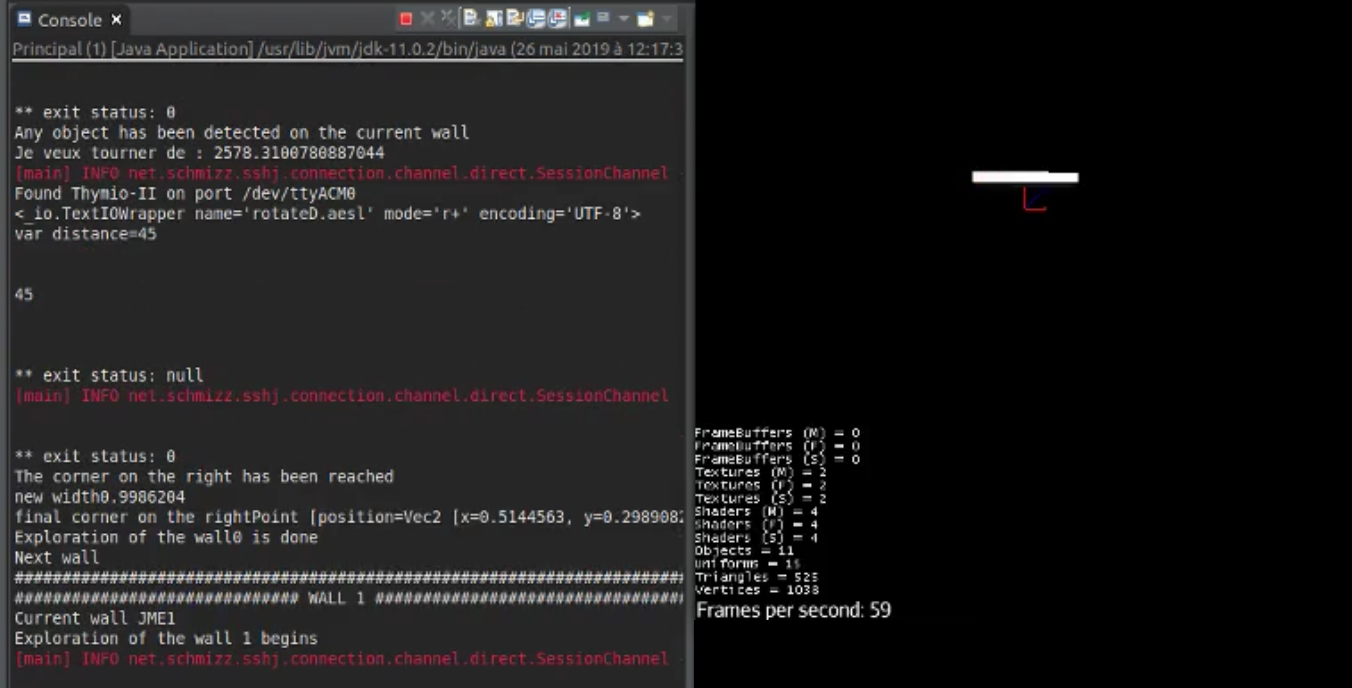
\includegraphics[scale=0.35]{instanceApp.png}
		\caption{An instance of the robot's exploration}
	\end{center}
\end{figure}

\end{document}